\subsection{\cinterface}
\label{sec:client_interface}

The client interface is illustrated in figure \ref{fig:client_interface}.
After login, the \aclient[] is presented with the \textit{main} window. All the window have a back function who enables the user to return to the previous window.

\subsubsection{Main}
The \aclient[] main window have three buttons: ``Add problem'', ``My problems'' and ``Search for problems''.
The ``Add problem'' button sends the user to the ``Categorize new problem'' window.
The ``My problems'' and ``Search for problems'' button sends the user to ``Search'' window.

\subsubsection{Search}
The search window contains a search button, a list where found problems are displayed, a settings and the frame ``Categories and tags''
The search button will start a search with the current configuration and show the results in the list. A problem can be double clicked to view details about the problem in the ``Client problem view'' windows.

\paragraph{Categories and tags} 
This frame is used in a few other windows. 
The frame contains a list of categories, when a category is selected the tags connected to it is shown.  

\subsubsection{Client problem view}
This window contains information about the selected problem. There is a info field which contains relevant information about the problem e.g. the description of the problem, a subscription check-box which is not visible for the user who created the problem, a text field with all the previous entered comments if any, a field to write new comments in, a button called ``Add comment'' to submit the new comment and a field with non or more solutions written by the staff members.  

\subsubsection{Categorize New Problem}
This window contains the frame ``Categories and tags'' and a search button. When a search is conducted the window ``Search for similar problems'' is opened. 

\subsubsection{Search for similar problems}
The ``Search for similar problems'' contains a button called ``No suitable problem found'' and the window ``Search'' which contains the frame ``Categories and tags''.
This window is actually just ``Search'' with an additional button added. The search results showed in the ``Problems found'' column can be selected and the window ``Client problem view'' is shown. The button ``No suitable problem found'' directs the user to ``Create new problem''. 


\subsubsection{Create new problem}
The ``Create new problem'' window's purpose is to describe, categorize and submit a problem. The frame ``Categories and tags'' enables the \aclient to pick what tags describe the problem best, the text field is used to write a description of the problem. When the ``Add problem'' is pressed the problem is send and the user is directed to the ``Client problem view'' where he can see the final description of the problem and relevant statistics.    




\begin{comment} %%%%%%%%%%%%%%%%%%%COMMENT



The client interface is illustrated in figure \ref{fig:client_interface}.
After login, the \aclient[] is presented with the \textit{main} screen, which gives four possibilities:
\fixme{hvis client ikke skal kunne tilg� statistics s� skal dette stykke �ndres}
%After login, the \aclient[] is greeted with the \textit{main} screen, wich gives three posebilities:
\begin{itemize}
	\item Add problem
	\item My problems
	\item Search for problem(s)
	\item Statistics
\end{itemize}

The four options reflect the use cases of the \aclient[] in section \ref{sec:usage}
%These main possibilities are thoroughly described in the following sub-subsection, since they are the reflect the three use cases of the \aclient[] in section \ref{sec:usage}; submit problem, see all problems, and get statistics.
Due to the nature of our webbased system, the \aclient[] can anytime terminate the session and logout/close.


\subsubsection{Add Problem}
As the name indicates, this button initiates the process of adding a specific problem to the system.
%The process starts by selecting what kind of problem the \aclient[] has.

This is done by selecting \textit{tags} which describes the problem. Tags are grouped under categories. %Each tag can only exist under one category, however if the need arises, it is possible to create a duplicate tag under another category.\fixme{Er det smart at have to tags der hedder det samme?}
We say that the problem is ``categorized'' when it has tags associated with it.

When the \aclient[] is satisfied with the categorization of the problem, the ``Search'' button can be clicked, which will make the system search for problems with similar categorization, prioritizing \fixme{skriv om hvordan det g�res} the most relevant problems.
The \aclient[] is then presented with a list of all similar problems.

identical problems
similar problems with solution
similar problems without solution

 
If a similar problem is found, the \aclient[] has the option to \textit{``subcribe''} to the problem, making the \aclient[] receive all the same notifications as the person who created the problem.
This dramatically reduces redundancy in a case where multiple users has the same or similar problem.
This also saves the \aclient s the time to create and describe a new problem in the system.
If no suitable problem is found, the \aclient[] is allowed to describe his problem with words, as well as alter the tags which he/she selected earlier, in case he/she changed his/her mind.
Ultimately, the problem is added to the database after fully described. This process will initialize the workload monitor, for distributing the problem to a \astaff[] member, who is likely to solve the problem.

\subsubsection{My Problems}
This button navigates to a window where the problems created by the \aclient[] as well as the problems which the \aclient[] has subscribed to is shown.

\subsubsection{Search for Problem(s)}
Clicking this button will bring the \aclient[] to the problems search-screen, where he/she can search by specifying tags which possibly are attached to the problems that the \aclient[] wishes to find.

\subsubsection{Statistics}
\fixme{Der skal laves et interface til statistics, ellers det skal i hvert fald beskrives.}

\end{comment} %%%%%%%%%%%%%%%%%%%COMMENT

\begin{figure}[htb]
\begin{center}
 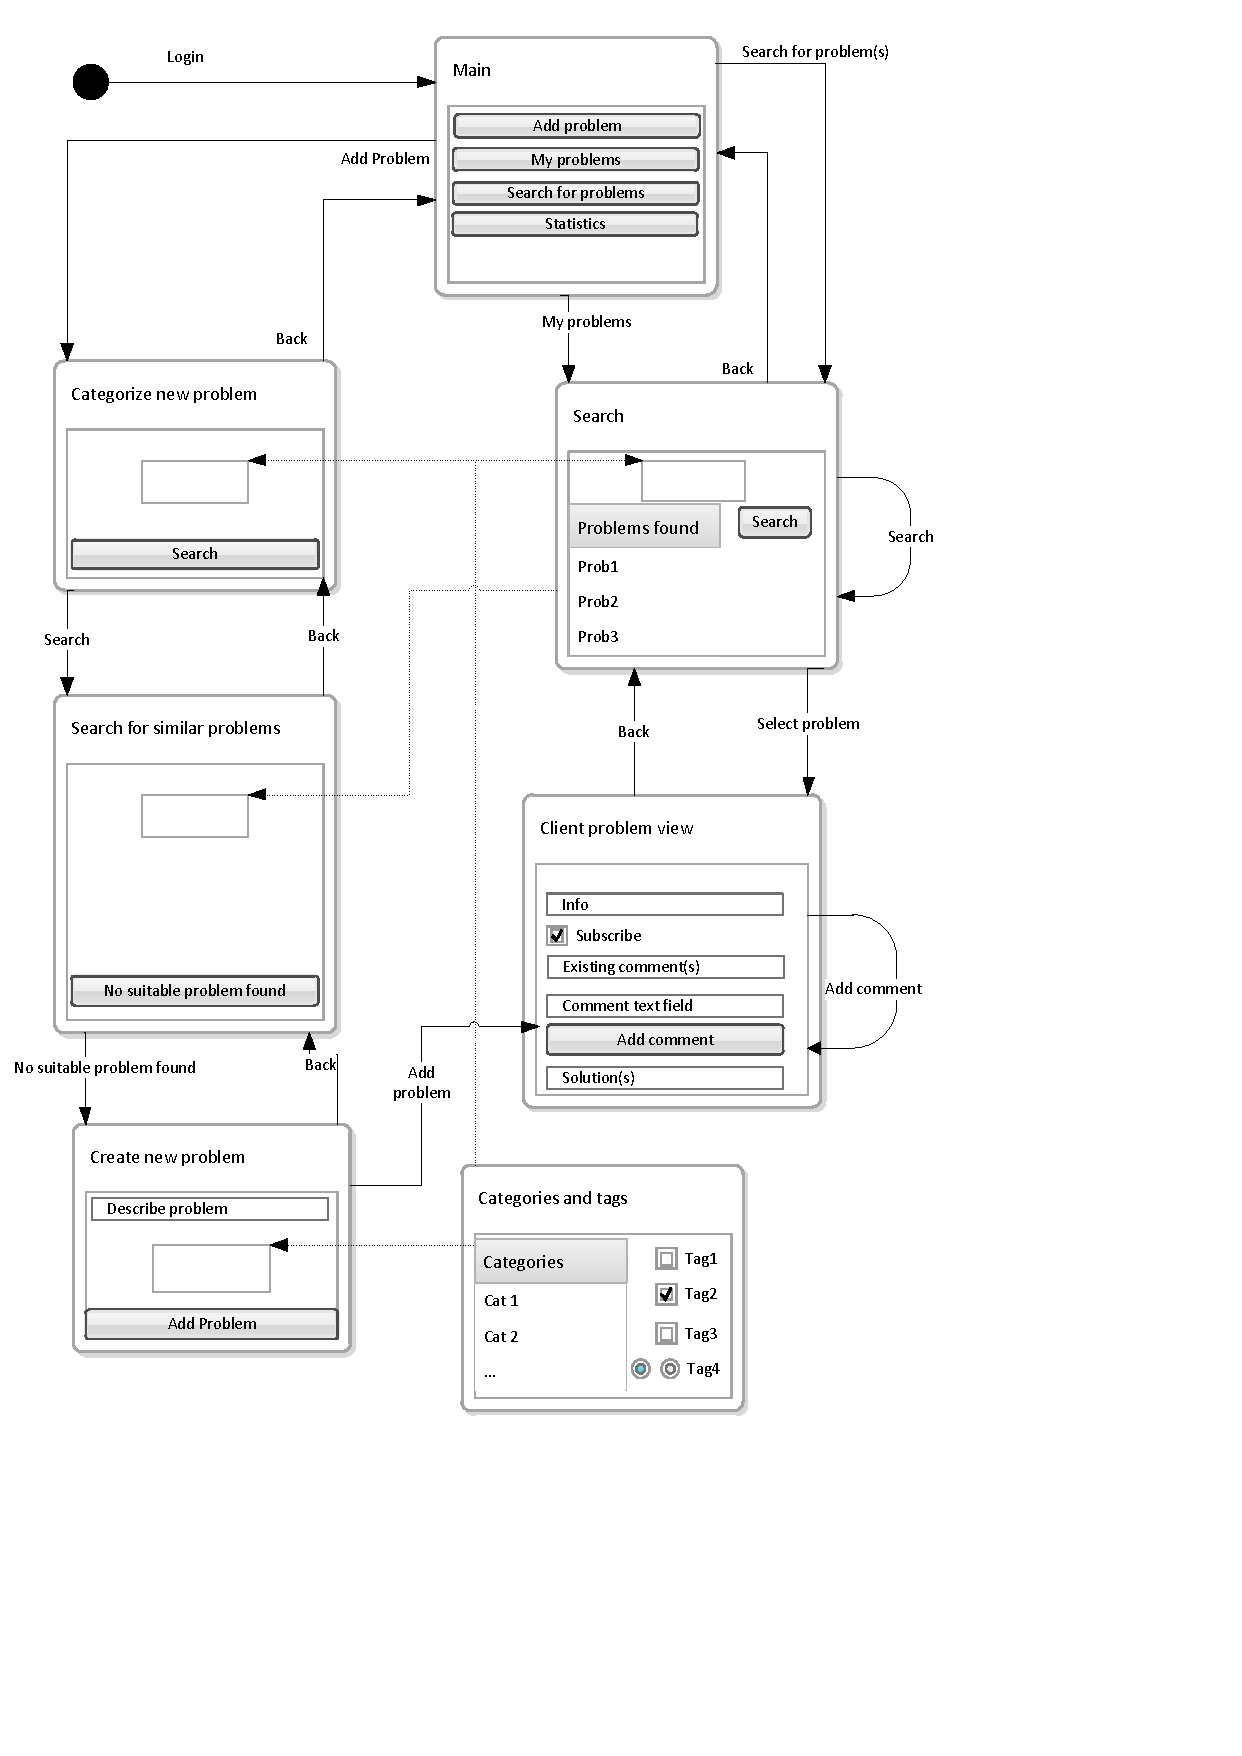
\includegraphics[width = \textwidth , clip=true, trim=0 5cm 5cm 0]{input/application_domain_analysis/Navigation_DiagramClient.pdf}
\morscaption{\cinterface[]}
\label{fig:client_interface}
\end{center}
\end{figure}




